\documentclass[11pt]{article}

\usepackage[a4paper,margin=1in]{geometry}
\usepackage[T1]{fontenc}
\usepackage[utf8]{inputenc}
\usepackage{lmodern}
\usepackage{microtype}
\usepackage{amsmath,amssymb,amsthm,mathtools,mathrsfs}
\usepackage{booktabs,array}
\usepackage{graphicx}
\usepackage{float}
\usepackage{placeins}
\usepackage{enumitem}
\usepackage[numbers,sort&compress]{natbib}
\usepackage{xcolor}
\usepackage{xurl}
\usepackage[colorlinks=true,linkcolor=blue!55!black,citecolor=blue!55!black,urlcolor=blue!65!black]{hyperref}
\usepackage[nameinlink,noabbrev]{cleveref}

\newtheorem{theorem}{Theorem}[section]
\newtheorem{proposition}[theorem]{Proposition}
\newtheorem{lemma}[theorem]{Lemma}
\newtheorem{corollary}[theorem]{Corollary}
\theoremstyle{remark}
\newtheorem{remark}[theorem]{Remark}
\newtheorem{definition}[theorem]{Definition}

\newcommand{\cK}{\mathcal K}
\newcommand{\cB}{\mathcal B}
\newcommand{\cQ}{\mathcal Q}
\newcommand{\cP}{\mathcal P}
\newcommand{\cI}{\mathcal I}
\newcommand{\R}{\mathbb R}
\newcommand{\norm}[1]{\left\lVert#1\right\rVert}
\newcommand{\HS}{\mathfrak S_2}
\newcommand{\TC}{\mathfrak S_1}
\newcommand{\uc}{u_{\mathrm c}}
\newcommand{\rhop}{\rho_{\mathrm c}}
\newcommand{\Qper}{\cQ_{\mathrm{per},\sigma}}

\title{Endpoint Spikes, Logarithmic Peripheral Conditioning,\\
and Continuum-Anchored Small-Noise Deflation}
\author{Liang Wang}
\date{July 2026}

\begin{document}
\maketitle

\begin{abstract}
The fixed-noise Perron and negative-parity branches of the folded-Gaussian
band-merging operator have validated intrinsic weighted Riesz kernels.  The
next question is whether their $L^2$ contour theory can remain uniformly
conditioned as the noise width $\sigma$ tends to zero.  It cannot.

Let $\pi_\sigma$ be the stationary density and let $g_\sigma$ be the signed
left density of the negative branch.  We prove the mesoscopic endpoint law
\[
 \sqrt t\,\pi_\sigma(1-t),
 \quad -\sqrt t\,g_\sigma(1-t)
 \longrightarrow
 c_R:=\frac{\rho_{\mathrm c}}{2\sqrt{u_{\mathrm c}}}
 =0.226423589260506\ldots
\]
whenever $t\downarrow0$ and $\sigma/t\to0$.  Together with the finite
postcritical spike majorants, this gives
\[
 \norm{\pi_\sigma}_2,\ \norm{g_\sigma}_2,\
 \norm{\cP_{+,\sigma}}_{\HS},\
 \norm{\cP_{-,\sigma}}_{\HS}
 =\Theta\!\left(\sqrt{\log(1/\sigma)}\right).
\]
For every fixed-radius isolating circle, the contour resolvent is therefore
at least of this order.  Thus a uniform $O(1)$ $L^2$ resolvent theorem is
impossible.  This lower bound does not determine the reduced-resolvent upper.

The same endpoint structure provides a bypass.  Direct differentiation of
the rank-two weighted kernel gives
\[
 \norm{E_n\cQ_{\mathrm{per},\sigma}E_n
       -\cQ_{\mathrm{per},\sigma}}_{\HS}
 =O(n^{-1}\sigma^{-3/2}),
\]
where $E_n$ is orthogonal cell averaging.  Hence the continuum-anchored bulk
\[
 \widetilde B_{n,\sigma}
 =E_n\cK_\sigma E_n-E_n\cQ_{\mathrm{per},\sigma}E_n
 =E_n\cB_\sigma E_n
\]
satisfies
\[
 \norm{\widetilde B_{n,\sigma}^2-\cB_\sigma^2}_{\TC}
 =O(n^{-1}\sigma^{-2})+O(n^{-2}\sigma^{-3}).
\]
Thus $n\sigma^2\to\infty$ still suffices.  The remaining spectral gate is the
intrinsic identification defect between the finite matrix's own weighted
Riesz term and the compression of the continuum term.  A
$204800$-dimensional floating audit supports the logarithmic law but is not
part of the proof.  No arithmetic trace formula, Hilbert--P\'olya operator,
or Riemann-hypothesis claim is made.
\end{abstract}

\noindent\textbf{Keywords:} small noise; Riesz projection; endpoint spike;
resolvent conditioning; Hilbert--Schmidt operator; Galerkin deflation.

\noindent\textbf{MSC 2020:} 47A10; 47B10; 37M25; 37C30; 65R20.

\section{Introduction}

For a fixed positive Gaussian width, the Perron and negative-parity
eigenvalues of the folded quadratic Markov operator can be isolated by
explicit Euclidean contours.  Their weighted Riesz terms are gauge-free,
rank one, and have smooth Hilbert--Schmidt kernels
\citep{WangRieszBridge2026,WangEuclideanContour2026,WangRankTwo2026}.
Subtracting them gives the intrinsic bulk
\begin{equation}
 \cB_\sigma
 =\cK_\sigma-\cQ_{+,\sigma}-\cQ_{-,\sigma}.
 \label{eq:bulk}
\end{equation}
At $\sigma=10^{-2}$, full and adaptive discretizations converge to this
bulk in Hilbert--Schmidt norm, and their squares converge in trace norm.

The small-noise problem separates spatial resolution from spectral
conditioning.  The raw Gaussian kernel obeys
\begin{equation}
 \norm{\cK_\sigma}_{\HS}=O(\sigma^{-1/2}),
 \qquad
 \norm{E_n\cK_\sigma E_n-\cK_\sigma}_{\HS}
 =O(n^{-1}\sigma^{-3/2}).
 \label{eq:raw-mesh}
\end{equation}
Consequently $n\sigma^2\to\infty$ is sufficient for the raw two-step
trace-ideal limit \citep{WangSmallNoiseMesh2026}.  Extending that theorem to
the intrinsic bulk was left under a uniform peripheral transport condition.
The coarsest proposed route assumed that the continuum and discrete contour
resolvents were $O(\sigma^{-\beta})$ and paid for two resolvents in the first
resolvent identity.

The present paper shows that interpreting $\beta=0$ as a uniform $O(1)$
$L^2$ contour is already excluded by the invariant density.  The
deterministic Misiurewicz density has one-sided square-root spikes.  Gaussian
smoothing cuts each spike off at distance $O(\sigma)$, and the squared
density accumulates a logarithm between $\sigma$ and a fixed macroscopic
scale.  The Riesz projection itself therefore becomes ill-conditioned in
$L^2$, even though its eigenvalue remains isolated in the natural
tower/spike space.

This is not a contradiction.  Keller--Liverani stability is a two-norm
statement on a strong dynamical space and a weak $L^1$ space
\citep{KellerLiverani1999}.  The $L^2$ norm sees the increasingly sharp
postcritical density spikes.  Spectral isolation and Hilbert-space
conditioning are different questions.

The logarithmic obstruction can nevertheless be bypassed for the spatial
part of the problem.  Instead of comparing two Riesz integrals with two
large resolvents, we differentiate the already identified rank-one kernels.
Their target derivatives have the same $\sigma^{-3/2}$ scale as the raw
Gaussian kernel.  Orthogonal cell averaging then preserves the $p>2$
two-step mesh law for the continuum-anchored bulk.

The outcome is a sharper map of the remaining maze:
\begin{enumerate}[label=\textbf{G\arabic*.},leftmargin=3em]
 \item fixed-geometry $O(1)$ $L^2$ resolvents are impossible;
 \item peripheral kernel size grows only logarithmically, hence more slowly
       than every negative power of $\sigma$;
 \item spatial compression of the continuum peripheral kernel is controlled
       at the raw Markov exponent $n^{-1}\sigma^{-3/2}$;
 \item the unresolved quantity is only the identification of the actual
       finite-matrix Riesz term with that compressed continuum kernel.
\end{enumerate}

\section{Operator and peripheral factors}
\label{sec:operator}

Let
\begin{equation}
 f(x)=1-\uc x^2,
 \qquad
 \uc=1.543689012692076\ldots,
 \label{eq:map}
\end{equation}
where $\uc$ is the first band-merging parameter.  On the folded state space
$I=[0,1]$, put
\begin{equation}
 k_\sigma(x,y)
 =\frac{\phi_\sigma(y-f(x))+\phi_\sigma(-y-f(x))}
 {Z_\sigma(x)},
 \quad
 Z_\sigma(x)=\int_0^1
 \{\phi_\sigma(y-f(x))+\phi_\sigma(-y-f(x))\}\,dy,
 \label{eq:kernel}
\end{equation}
where
$\phi_\sigma(s)=(2\pi\sigma^2)^{-1/2}e^{-s^2/(2\sigma^2)}$.
The Markov operator on observables is
\begin{equation}
 (\cK_\sigma v)(x)=\int_0^1k_\sigma(x,y)v(y)\,dy.
 \label{eq:operator}
\end{equation}
It is compact and strongly positive for every $\sigma>0$.

Let $\pi_\sigma$ be the stationary density,
\begin{equation}
 \cK_\sigma^*\pi_\sigma=\pi_\sigma,
 \qquad
 \int_0^1\pi_\sigma=1.
 \label{eq:stationary}
\end{equation}
The small-noise parity theorem supplies a simple real eigenvalue
$\lambda_-(\sigma)\to-1$, a right observable $h_\sigma$, and a signed left
density $g_\sigma$ such that
\begin{equation}
 \cK_\sigma h_\sigma=\lambda_-(\sigma)h_\sigma,
 \quad
 \cK_\sigma^*g_\sigma=\lambda_-(\sigma)g_\sigma,
 \quad
 \int_0^1h_\sigma g_\sigma=1.
 \label{eq:parity-factors}
\end{equation}
The normalization is chosen so that $h_\sigma$ tends to $+1$ on the central
component and to $-1$ on the outer component.  The signed density tends in
$L^1$ to the deterministic signed component density
\citep{WangBoundaryLayer2026}.

The Riesz projections and weighted terms have exact kernels
\begin{align}
 p_{+,\sigma}(x,y)&=\pi_\sigma(y),
 &q_{+,\sigma}(x,y)&=\pi_\sigma(y),
 \label{eq:perron-kernel}\\
 p_{-,\sigma}(x,y)&=h_\sigma(x)g_\sigma(y),
 &q_{-,\sigma}(x,y)&=\lambda_-(\sigma)h_\sigma(x)g_\sigma(y).
 \label{eq:parity-kernel}
\end{align}
Their sum is denoted
\begin{equation}
 \Qper=\cQ_{+,\sigma}+\cQ_{-,\sigma}.
 \label{eq:qper}
\end{equation}

The deterministic central density has the form
\begin{equation}
 \rho_D(x)=\frac{v(x)}{\pi\sqrt{r^2-x^2}},
 \qquad r=\uc-1,
 \label{eq:central-density}
\end{equation}
where $v$ is positive and analytic.  Its value at the critical point is
\begin{equation}
 \rhop=\rho_D(0)=0.562641254486572\ldots.
 \label{eq:rho-c}
\end{equation}

\section{The mesoscopic endpoint law}
\label{sec:mesoscopic}

The preceding boundary-layer theorem resolved the microscopic scale
$1-y=O(\sigma)$.  For fixed $\xi\ge0$ it gives
\begin{equation}
 \sqrt\sigma\,\pi_\sigma(1-\sigma\xi)\longrightarrow R(\xi),
 \qquad
 -\sqrt\sigma\,g_\sigma(1-\sigma\xi)\longrightarrow R(\xi),
 \label{eq:microscopic-profile}
\end{equation}
where the stationary statement follows by the same positive eigenrelation,
and
\begin{equation}
 R(\xi)=\rhop\int_0^\infty
 \frac{\phi(\uc q^2-\xi)}{\Phi(\uc q^2)}\,dq,
 \qquad
 R(\xi)\sim\frac{\rhop}{2\sqrt{\uc\xi}}.
 \label{eq:R-profile}
\end{equation}
The next theorem makes the overlap with the deterministic spike uniform.

\begin{theorem}[Mesoscopic endpoint matching]
\label{thm:mesoscopic}
Let $t=t(\sigma)$ satisfy
\begin{equation}
 t\longrightarrow0,
 \qquad
 \frac{\sigma}{t}\longrightarrow0.
 \label{eq:mesoscopic-regime}
\end{equation}
Then
\begin{equation}
 \sqrt t\,\pi_\sigma(1-t)\longrightarrow c_R,
 \qquad
 -\sqrt t\,g_\sigma(1-t)\longrightarrow c_R,
 \qquad
 c_R=\frac{\rhop}{2\sqrt\uc}.
 \label{eq:mesoscopic-law}
\end{equation}
The convergence is uniform on every overlap window
\begin{equation}
 \sigma^a\le t\le\delta,
 \qquad 0<a<1,
 \label{eq:overlap-window}
\end{equation}
after first taking $\sigma\downarrow0$ and then $\delta\downarrow0$.
\end{theorem}

\begin{proof}
Put $y=1-t$.  The only sources that reach $y$ without an exponentially
unlikely jump lie near the positive critical preimage
\begin{equation}
 x_t=\sqrt{t/\uc}.
 \label{eq:critical-preimage}
\end{equation}
Since $t/\sigma\to\infty$, this source is many Gaussian widths from the
conditioned target boundary.  Hence $Z_\sigma(x)=1+o(1)$ uniformly on the
relevant source window.  Write
\begin{equation}
 x=x_t+\frac{\sigma s}{2\sqrt{\uc t}}.
 \label{eq:source-scaling}
\end{equation}
Then
\begin{equation}
 \frac{\uc x^2-t}{\sigma}=s+o(1),
 \qquad
 dx=\frac{\sigma}{2\sqrt{\uc t}}\,ds.
 \label{eq:source-jacobian}
\end{equation}
Stochastic stability and regularity on the central component give
$\pi_\sigma(x)=\rhop+o(1)$ uniformly on this window.  Gaussian tails permit
restriction to bounded $s$ before sending the bound to infinity.  The first
term in \eqref{eq:kernel} therefore gives
\begin{equation}
 \pi_\sigma(1-t)
 =\frac{\rhop+o(1)}{2\sqrt{\uc t}}\int_\R\phi(s)\,ds
 =\frac{\rhop+o(1)}{2\sqrt{\uc t}}.
 \label{eq:stationary-laplace}
\end{equation}
The folded second Gaussian and all other sources are exponentially small.

For the signed density,
\begin{equation}
 \lambda_-(\sigma)g_\sigma(y)
 =\int_0^1g_\sigma(x)k_\sigma(x,y)\,dx.
 \label{eq:g-eigenrelation}
\end{equation}
On the central source window,
$g_\sigma(x)=\rhop+o(1)$, while
$\lambda_-(\sigma)\to-1$.  Repeating the same calculation proves the second
limit with the negative sign.

For $\sigma^a\le t\le\delta$, the relative Taylor error in
\eqref{eq:source-jacobian} is $O(\sigma/t)$, hence uniformly small.  The
central source tends uniformly to zero as $\delta\downarrow0$, and Gaussian
tail bounds remain uniform.  This proves the overlap statement.
\end{proof}

Numerically,
\begin{equation}
 c_R=0.22642358926050635\ldots,
 \qquad
 c_R^2=0.05126764177361048\ldots.
 \label{eq:cR-numerical}
\end{equation}
The second number is the endpoint contribution per unit logarithmic scale to
the squared $L^2$ norm.

\section{Logarithmic Riesz conditioning}
\label{sec:conditioning}

The tower/spike estimates for a postcritically finite Misiurewicz map give a
finite collection of local bounds
\begin{equation}
 |\pi_\sigma(s+\sigma\xi)|
 +|g_\sigma(s+\sigma\xi)|
 \le C\sigma^{-1/2}(1+|\xi|)^{-1/2}
 \label{eq:spike-majorant}
\end{equation}
near every one-sided square-root spike $s$, and a uniform bound on their
complement \citep{Misiurewicz1981,KellerNowicki1992,Baladi2000,
WangBoundaryLayer2026}.  Squaring and integrating gives an upper logarithm.
The endpoint matching theorem gives the lower logarithm.

\begin{theorem}[Logarithmic left-factor law]
\label{thm:left-log}
As $\sigma\downarrow0$,
\begin{equation}
 \norm{\pi_\sigma}_{L^2}^2=\Theta(\log(1/\sigma)),
 \qquad
 \norm{g_\sigma}_{L^2}^2=\Theta(\log(1/\sigma)).
 \label{eq:left-log}
\end{equation}
Moreover the endpoint alone satisfies
\begin{equation}
 \liminf_{\sigma\downarrow0}
 \frac{\norm{\pi_\sigma}_{L^2}^2}{\log(1/\sigma)}
 \ge c_R^2,
 \qquad
 \liminf_{\sigma\downarrow0}
 \frac{\norm{g_\sigma}_{L^2}^2}{\log(1/\sigma)}
 \ge c_R^2.
 \label{eq:endpoint-liminf}
\end{equation}
\end{theorem}

\begin{proof}
Integrating \eqref{eq:spike-majorant} over the finitely many spike
neighborhoods yields
\begin{equation}
 \norm{\pi_\sigma}_2^2+\norm{g_\sigma}_2^2
 \le C\log(1/\sigma).
 \label{eq:log-upper}
\end{equation}
For the lower bound, fix $0<a<1$.  On
$\sigma^a\le t\le\delta$, \cref{thm:mesoscopic} gives, after shrinking
$\delta$,
\[
 \pi_\sigma(1-t)^2,\ g_\sigma(1-t)^2
 \ge(c_R-o(1))^2t^{-1}.
\]
Its integral is
\[
 a c_R^2\log(1/\sigma)+o(\log(1/\sigma)).
\]
Letting $a\uparrow1$ proves \eqref{eq:endpoint-liminf} and the lower half of
\eqref{eq:left-log}.
\end{proof}

The right parity observable satisfies
\begin{equation}
 0<c\le\norm{h_\sigma}_{L^2}\le
 \norm{h_\sigma}_{L^\infty}\le C.
 \label{eq:h-bounds}
\end{equation}
Indeed, spectral stability gives convergence to the component-sign
observable away from its $O(\sigma)$ transition layer; the exact
error-function profile controls that layer \citep{WangBoundaryLayer2026}.

\begin{corollary}[Peripheral Riesz growth]
\label{cor:projector-log}
The simple Riesz projections and weighted terms satisfy
\begin{align}
 \norm{\cP_{+,\sigma}}_{\HS}
 &=\norm{\pi_\sigma}_2
 =\Theta(\sqrt{\log(1/\sigma)}),
 \label{eq:perron-projector-log}\\
 \norm{\cP_{-,\sigma}}_{\HS}
 &=\norm{h_\sigma}_2\norm{g_\sigma}_2
 =\Theta(\sqrt{\log(1/\sigma)}),
 \label{eq:parity-projector-log}\\
 \norm{\Qper}_{\HS}
 &=O(\sqrt{\log(1/\sigma)}).
 \label{eq:qper-log}
\end{align}
Thus the peripheral size has regular-variation index zero: it is
$O(\sigma^{-\epsilon})$ for every $\epsilon>0$, but it is not $O(1)$.
\end{corollary}

\begin{proof}
Equations \eqref{eq:perron-kernel}--\eqref{eq:parity-kernel} are rank-one
kernels, so their Hilbert--Schmidt norms factor exactly.  Since
$|\lambda_-(\sigma)|\to1$, \cref{thm:left-log} and
\eqref{eq:h-bounds} prove the first two statements.  The third follows by
the triangle inequality.
\end{proof}

\subsection{The fixed-contour resolvent obstruction}

Let $\Gamma$ be a circle of radius $r_\Gamma$ that isolates one peripheral
branch for all sufficiently small $\sigma$.  Such fixed geometry is
compatible with strong/weak perturbation theory; the obstruction below
concerns its $L^2$ norm, not its existence.

\begin{theorem}[No uniform fixed-geometry $L^2$ resolvent]
\label{thm:resolvent-lower}
For either peripheral circle,
\begin{equation}
 \sup_{z\in\Gamma}\norm{(z-\cK_\sigma)^{-1}}_{L^2\to L^2}
 \ge
 \frac{1}{r_\Gamma}\norm{\cP_{\pm,\sigma}}_{L^2\to L^2}
 \ge c\sqrt{\log(1/\sigma)}.
 \label{eq:resolvent-lower}
\end{equation}
In particular, no $O(1)$ $L^2$ contour-resolvent theorem is possible on
fixed-radius circles.
\end{theorem}

\begin{proof}
The Riesz formula and the arclength of a circle give
\begin{equation}
 \norm{\cP_{\pm,\sigma}}
 \le r_\Gamma
 \sup_{z\in\Gamma}\norm{(z-\cK_\sigma)^{-1}}.
 \label{eq:riesz-circle}
\end{equation}
For a rank-one operator, the operator and Hilbert--Schmidt norms agree.
Apply \cref{cor:projector-log}.
\end{proof}

\begin{remark}[What is not proved]
\label{rem:reduced-resolvent}
The lower bound \eqref{eq:resolvent-lower} comes entirely from the residue.
It does not upper-bound the reduced resolvent on the complementary spectral
subspace.  Nonnormal pseudospectral growth may be larger
\citep{GohbergKrein1969,Kato1995}.  Thus this paper disproves uniform $O(1)$
conditioning but does not identify a matching upper or a polynomial exponent
$\beta$ for the complete resolvent.
\end{remark}

\section{Direct peripheral-kernel resolution}
\label{sec:kernel-resolution}

The resolvent obstruction does not force a worse spatial mesh exponent.
The already isolated weighted term has a rank-two kernel whose derivatives
can be estimated from the eigenrelations without differentiating a contour
resolvent.

\begin{lemma}[Gaussian row derivative bounds]
\label{lem:gaussian-derivatives}
For sufficiently small $\sigma$,
\begin{align}
 \sup_x\norm{\partial_y k_\sigma(x,\cdot)}_{L^2_y}
 &\le C\sigma^{-3/2},
 \label{eq:target-row-derivative}\\
 \sup_x\int_0^1|\partial_x k_\sigma(x,y)|\,dy
 &\le C\sigma^{-1}.
 \label{eq:source-row-variation}
\end{align}
\end{lemma}

\begin{proof}
For an unconditioned normalized Gaussian, the first derivative has $L^2$
scale $\sigma^{-3/2}$ and total-variation scale $\sigma^{-1}$.  Folding adds
two terms.  Differentiating the row normalizer contributes the same scales.
Near a conditioned endpoint, the normalizer is bounded below by a positive
Gaussian half-mass in normalized coordinates; away from the endpoint it
tends to one.  Finally $f'$ is uniformly bounded.  These are the
normalized-kernel versions of the explicit Gaussian moment bounds in
\citep{WangSmallNoiseMesh2026}.
\end{proof}

\begin{proposition}[Peripheral derivative envelope]
\label{prop:peripheral-derivatives}
The left densities and right parity observable satisfy
\begin{align}
 \norm{\pi_\sigma'}_2+\norm{g_\sigma'}_2
 &=O(\sigma^{-3/2}),
 \label{eq:left-derivatives}\\
 \norm{h_\sigma'}_2&=O(\sigma^{-1}).
 \label{eq:right-derivative}
\end{align}
Consequently the rank-two weighted kernel $q_{\mathrm{per},\sigma}$ obeys
\begin{align}
 \norm{\partial_x q_{\mathrm{per},\sigma}}_{L^2(I^2)}
 &=O\!\left(\sigma^{-1}\sqrt{\log(1/\sigma)}\right),
 \label{eq:q-source}\\
 \norm{\partial_y q_{\mathrm{per},\sigma}}_{L^2(I^2)}
 &=O(\sigma^{-3/2}).
 \label{eq:q-target}
\end{align}
\end{proposition}

\begin{proof}
Differentiate \eqref{eq:stationary} and the left equation in
\eqref{eq:parity-factors}.  Minkowski's inequality,
\cref{lem:gaussian-derivatives},
$\norm{\pi_\sigma}_1=1$, and the uniform $L^1$ bound for $g_\sigma$ give
\eqref{eq:left-derivatives}.  Differentiating the right equation in
\eqref{eq:parity-factors}, using \eqref{eq:source-row-variation},
\eqref{eq:h-bounds}, and $|\lambda_-(\sigma)|\ge1/2$ gives
\eqref{eq:right-derivative}.

Differentiating \eqref{eq:perron-kernel} and
\eqref{eq:parity-kernel}, rank-one factorization gives
\[
 \norm{\partial_xq_{-,\sigma}}_2
 =|\lambda_-|\norm{h_\sigma'}_2\norm{g_\sigma}_2,
 \qquad
 \norm{\partial_yq_{-,\sigma}}_2
 =|\lambda_-|\norm{h_\sigma}_2\norm{g_\sigma'}_2.
\]
The Perron source derivative vanishes and its target derivative is
$\pi_\sigma'$.  Apply \cref{thm:left-log}.
\end{proof}

Let $E_n$ denote orthogonal averaging on the $n$ equal cells of $I$.
The tensor cell average of a kernel represents $E_nTE_n$.

\begin{theorem}[Peripheral cell-average resolution]
\label{thm:peripheral-projection}
The compressed continuum weighted term satisfies
\begin{equation}
 \boxed{
 \norm{E_n\Qper E_n-\Qper}_{\HS}
 =O(n^{-1}\sigma^{-3/2}).}
 \label{eq:peripheral-projection}
\end{equation}
\end{theorem}

\begin{proof}
The one-dimensional Poincar\'e--Wirtinger inequality on each cell, applied
successively in the two variables, gives
\begin{equation}
 \norm{E_nTE_n-T}_{\HS}
 \le\frac{1}{\pi n}
 \left(\norm{q_x}_{L^2(I^2)}+\norm{q_y}_{L^2(I^2)}\right).
 \label{eq:kernel-poincare}
\end{equation}
Insert \eqref{eq:q-source}--\eqref{eq:q-target} and use
$\sqrt{\log(1/\sigma)}=O(\sigma^{-1/2})$.
\end{proof}

\section{Continuum-anchored bulk-square convergence}
\label{sec:anchored}

Define the continuum intrinsic bulk by \eqref{eq:bulk} and its anchored
Galerkin compression by
\begin{align}
 \widetilde B_{n,\sigma}
 &:=E_n\cK_\sigma E_n-E_n\Qper E_n
 \notag\\
 &=E_n\cB_\sigma E_n.
 \label{eq:anchored-bulk}
\end{align}
This is an exact algebraic identity.  The term \emph{anchored} emphasizes
that the peripheral kernel comes from the continuum operator, not from a
new diagonalization of the finite matrix.

\begin{theorem}[Anchored small-noise mesh law]
\label{thm:anchored-mesh}
Uniformly for sufficiently small $\sigma$,
\begin{align}
 \norm{\cB_\sigma}_{\HS}&=O(\sigma^{-1/2}),
 \label{eq:bulk-size}\\
 \norm{\widetilde B_{n,\sigma}-\cB_\sigma}_{\HS}
 &=O(n^{-1}\sigma^{-3/2}),
 \label{eq:anchored-hs}\\
 \norm{\widetilde B_{n,\sigma}^2-\cB_\sigma^2}_{\TC}
 &=O(n^{-1}\sigma^{-2})+O(n^{-2}\sigma^{-3}).
 \label{eq:anchored-trace}
\end{align}
In particular,
\begin{equation}
 n(\sigma)\sigma^2\longrightarrow\infty
 \label{eq:p-two-condition}
\end{equation}
is sufficient for anchored bulk-square trace-norm convergence.  For
$n(\sigma)\asymp\sigma^{-p}$, every $p>2$ closes the theorem.
\end{theorem}

\begin{proof}
The raw Markov bounds \eqref{eq:raw-mesh} and
\eqref{eq:qper-log} give
\[
 \norm{\cB_\sigma}_{\HS}
 \le O(\sigma^{-1/2})+O(\sqrt{\log(1/\sigma)})
 =O(\sigma^{-1/2}).
\]
Add the raw cell-average error in \eqref{eq:raw-mesh} to
\cref{thm:peripheral-projection} to obtain \eqref{eq:anchored-hs}.
Products of Hilbert--Schmidt operators are trace class, and
\begin{align}
 \norm{A_n^2-A^2}_{\TC}
 &\le\norm{A_n-A}_{\HS}
       (\norm{A_n}_{\HS}+\norm A_{\HS})
 \notag\\
 &\le\varepsilon(2\norm A_{\HS}+\varepsilon).
 \label{eq:hs-product}
\end{align}
With $\varepsilon=O(n^{-1}\sigma^{-3/2})$, this is
\eqref{eq:anchored-trace}.  Condition \eqref{eq:p-two-condition} sends both
terms to zero.
\end{proof}

The logarithmic peripheral growth therefore does not alter the raw Markov
power threshold.  It is asymptotically smaller than the
$\sigma^{-1/2}$ Hilbert--Schmidt size of the narrowing Gaussian kernel.

\section{The exact remaining identification defect}
\label{sec:identification}

Let
\begin{equation}
 G_{n,\sigma}=E_n\cK_\sigma E_n
 \label{eq:galerkin-markov}
\end{equation}
on the cell space.  When its two peripheral branches are intrinsically
identified, its actual finite-dimensional bulk is
\begin{equation}
 B_{n,\sigma}^{\mathrm{int}}
 =G_{n,\sigma}-\cQ_{\mathrm{per}}(G_{n,\sigma}).
 \label{eq:intrinsic-discrete-bulk}
\end{equation}

\begin{definition}[Intrinsic identification defect]
\label{def:identification}
Define
\begin{equation}
 \cI_{n,\sigma}
 :=\cQ_{\mathrm{per}}(G_{n,\sigma})
   -E_n\cQ_{\mathrm{per}}(\cK_\sigma)E_n.
 \label{eq:identification-defect}
\end{equation}
Then
\begin{equation}
 B_{n,\sigma}^{\mathrm{int}}-\widetilde B_{n,\sigma}
 =-\cI_{n,\sigma}.
 \label{eq:identification-identity}
\end{equation}
\end{definition}

\begin{corollary}[Sufficient intrinsic closure]
\label{cor:intrinsic-closure}
If
\begin{equation}
 \norm{\cI_{n,\sigma}}_{\HS}
 =O(n^{-1}\sigma^{-3/2}),
 \label{eq:identification-target}
\end{equation}
then \cref{thm:anchored-mesh} holds with
$B_{n,\sigma}^{\mathrm{int}}$ in place of
$\widetilde B_{n,\sigma}$.
\end{corollary}

\begin{proof}
Equation \eqref{eq:identification-identity} and the triangle inequality give
the same Hilbert--Schmidt rate.  Apply \eqref{eq:hs-product}.
\end{proof}

This isolates the remaining problem more sharply than a global peripheral
transport condition.  The spatial compression
\[
 E_n\cQ_{\mathrm{per}}(\cK_\sigma)E_n
 -\cQ_{\mathrm{per}}(\cK_\sigma)
\]
is already controlled by \cref{thm:peripheral-projection}.  Only the spectral
identification of the finite matrix's own Riesz term remains.  A proof should
target a reduced resolvent or a Feshbach/Grushin complement around the two
known factors.  Paying for two complete $L^2$ resolvents is sufficient but,
in view of \cref{thm:resolvent-lower}, structurally wasteful.

\section{Floating sparse audit}
\label{sec:numerics}

The theorem is analytic.  We nevertheless audit the predicted clocks on the
same row-normalized eight-sigma sparse family used in the preceding
small-noise studies.  The dimension is chosen by
\begin{equation}
 n\sigma\simeq20.48,
 \label{eq:numerical-resolution}
\end{equation}
and the calculation reaches $n=204800$ at $\sigma=10^{-4}$.
Right and left eigenvectors are normalized as in
\eqref{eq:parity-factors}.  All low-rank Hilbert--Schmidt and singular values
are evaluated from $2\times2$ Gram matrices; the full rank-two kernel is
never formed.

\begin{table}[H]
\centering
\small
\begin{tabular}{@{}rrrrrr@{}}
\toprule
$\sigma$ & $n$ & $\norm{P_+}_{\HS}$ & $\norm{P_-}_{\HS}$
& $\norm{Q_{\rm per}}_{\HS}$ & Perron resolvent lower\\
\midrule
$4\times10^{-3}$ & $5120$   & $1.15508$ & $1.14811$ & $1.63226$ & $23.1016$\\
$10^{-3}$        & $20480$  & $1.24273$ & $1.21532$ & $1.74451$ & $24.8547$\\
$2\times10^{-4}$ & $102400$ & $1.35334$ & $1.31207$ & $1.89259$ & $27.0667$\\
$10^{-4}$        & $204800$ & $1.40097$ & $1.35583$ & $1.95758$ & $28.0194$\\
\bottomrule
\end{tabular}
\caption{Floating peripheral-factor audit.  The resolvent column is the
algebraic lower formula $\norm{P_+}/0.05$ applied to floating projector data;
the data themselves are not validated enclosures.}
\label{tab:pilot}
\end{table}

Over the six smallest noise levels, least-squares fits of squared norms
against $\log(1/\sigma)$ give slopes
\begin{equation}
 0.17154\quad(P_+),
 \qquad
 0.14244\quad(P_-),
 \qquad
 0.31906\quad(Q_{\mathrm{per}}).
 \label{eq:fitted-slopes}
\end{equation}
These slopes include all postcritical spikes and are not identified with the
single-endpoint coefficient $c_R^2$.  The median mesoscopic coefficients at
$\sigma=10^{-4}$ are
\begin{equation}
 0.241782\quad(\pi_\sigma),
 \qquad
 0.245491\quad(-g_\sigma),
 \label{eq:observed-tail}
\end{equation}
compared with $c_R=0.226424$.  Their monotone drift is consistent with
\cref{thm:mesoscopic}.

\begin{figure}[H]
\centering
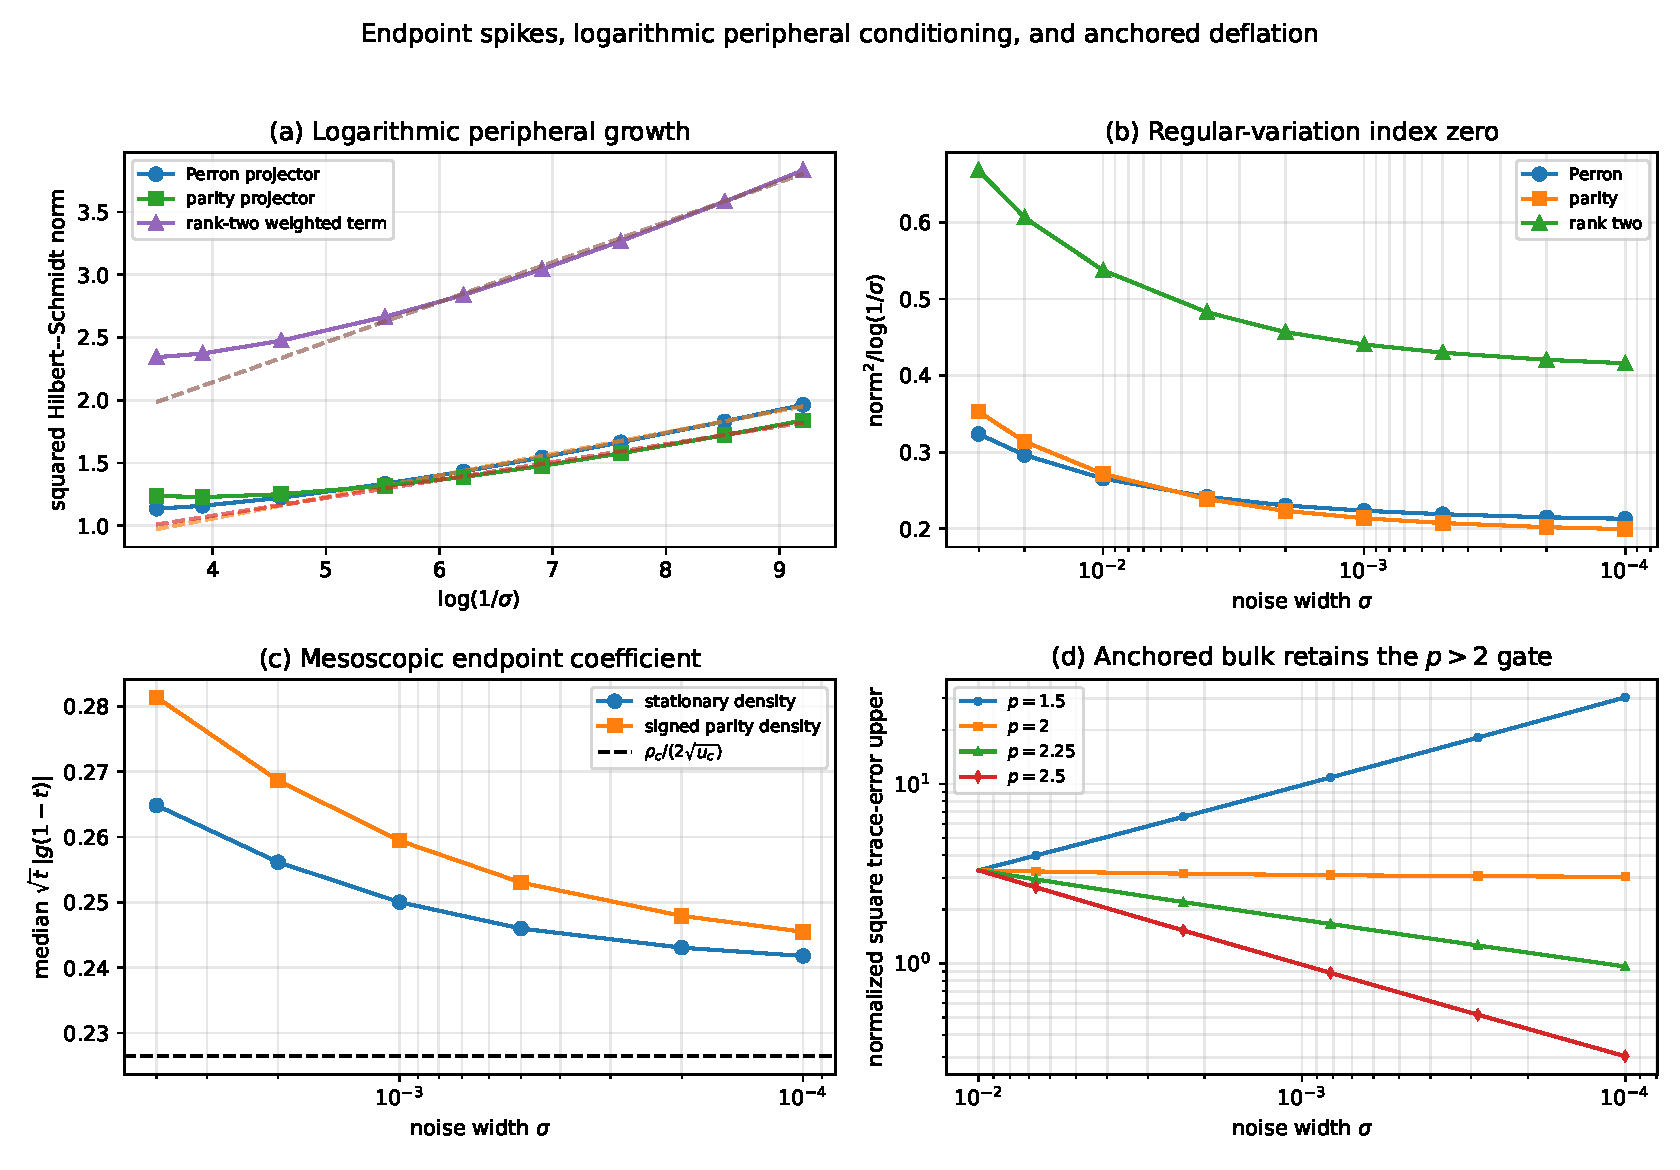
\includegraphics[width=\textwidth]{figures/logarithmic_peripheral_conditioning.pdf}
\caption{Logarithmic peripheral conditioning and the anchored bypass.
(a) Squared Perron, parity, and rank-two norms against $\log(1/\sigma)$,
with floating linear fits.  (b) Division by the logarithmic clock.  (c)
Mesoscopic endpoint coefficients approaching $c_R$.  (d) Normalized
anchored trace-error ledgers: $p=2$ is critical and every displayed $p>2$
decays.  Panels (a)--(c) are floating diagnostics; panel (d) displays the
proved exponents with unknown constants normalized to one.}
\label{fig:summary}
\end{figure}

The numerical data do not upper-bound a reduced resolvent and do not prove
\eqref{eq:identification-target}.  They test only the factor growth and
endpoint mechanism already isolated analytically.

\section{What is closed and what remains}
\label{sec:conclusion}

The small-noise contour gate has split into three distinct statements.
\begin{enumerate}[leftmargin=2.2em]
 \item \textbf{Spectral geometry.}  The Perron and negative branches remain
       simple and isolated on the natural dynamical space.  Their eigenvalue
       locations do not force a shrinking contour.
 \item \textbf{$L^2$ conditioning.}  Fixed-radius $O(1)$ resolvents are
       impossible because the residues themselves grow like
       $\sqrt{\log(1/\sigma)}$.
 \item \textbf{Spatial resolution.}  Direct rank-two kernel estimates bypass
       that obstruction and retain the $n\sigma^2\to\infty$ two-step law for
       continuum-anchored deflation.
\end{enumerate}

The next positive gate is precisely \eqref{eq:identification-target}.  A
useful proof should separate the logarithmic residue from the reduced
complement and transport the two known factors through a one-sided
Feshbach/Grushin system.  If that succeeds, the actual intrinsic finite
bulk---not only its continuum-anchored compression---inherits the $p>2$
small-noise theorem.

None of the present results identifies a dynamical trace with primes or
prime powers, constructs a self-adjoint operator, derives a $T\log T$
counting law, or locates a Riemann zero.  The result is an endpoint,
conditioning, and trace-ideal theorem for one explicit noisy transfer
family.

\section*{Data and code availability}

All source code, certificates, floating factor data, tests, figures, hashes,
and the manuscript are available in
\url{https://github.com/maris205/prime_dynamics_theory/tree/main/papers/RH-47-logarithmic-peripheral-conditioning}.

\bibliographystyle{plainnat}
\bibliography{references}

\end{document}
